\section{Graph Neural Networks (GNNs)}\label{sec:GNN_intro}

\subsection{The need for graph-based architectures}
Graph Neural Networks were theorized long before the machine learning revolution that saw them take center stage. The beginning of their rapid rise in both the international market and academic research can be traced back to the 2018 paper available at this here: \url{https://arxiv.org/abs/1806.01261}.

In the landscape of modern machine learning, different architectures are highly optimized to exploit the specific symmetries of their input data. For instance, CNNs are the standard for computer vision because they process data structured on a multi-index euclidean grid (like the pixels of an image). By sliding a shared kernel across the grid, CNNs naturally exploit \textit{spatial translation equivariance}. Similarly, Recurrent Neural Networks (RNNs) or LSTMs (which we will see later) operate on sequentially ordered data (like text files), exploiting \textit{time-shift equivariance}. Generally speaking, a function $F$ is said to be equivariant (or often, though less appropriately, invariant) under a transformation $T$ if $F(T(t)) = T(F(t))$. The CNN example is straightforward: if we have an algorithm that identifies a cat in an image by overlaying a mask on it, shifting the cat by one pixel will result in the mask shifting by the exact same amount. Try to independently apply this same reasoning to RNNs and temporal equivariance.

However, in many scientific and industrial applications, data does not easily fit into a rigid tensor structure or a strict sequential order (where the position of an element carries a fixed physical meaning), representing what is known as \textbf{sparse data}. Consider datasets such as social networks, economic interactions, molecular structures, the galactic web in astrophysics, or functional MRI brain activity maps. In HEP, a particle collision at the LHC produces a "spray" of particles known as a jet, while the measurements from tracking and calorimeter detectors naturally form a scattered point cloud, not an ordered grid. 

\begin{center}
    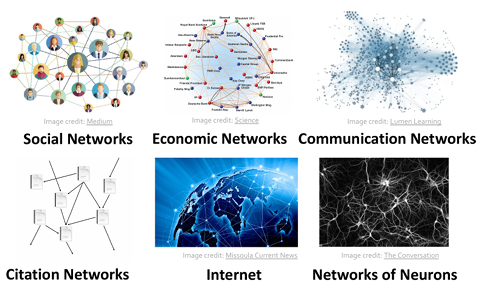
\includegraphics[width=0.32\textwidth]{figuresML/lesson_ml_5_pag_29a.png}
    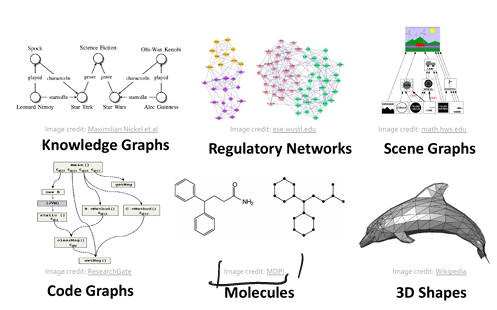
\includegraphics[width=0.32\textwidth]{figuresML/lesson_ml_5_pag_29b.png}
    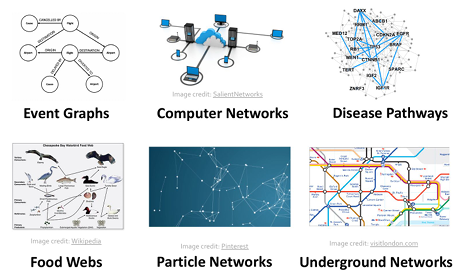
\includegraphics[width=0.32\textwidth]{figuresML/lesson_ml_5_pag_29c.png}
\end{center}

Attempting to cast this heterogeneous data into standard grid formats requires severe approximations, such as arbitrary binning (which leads to information loss) or the creation of highly sparse data structures filled primarily with zeros. To process this data natively, we require a structure that focuses on the nodes and their local connections, exploiting a new fundamental symmetry: \textbf{permutation equivariance} (or invariance). Because a point cloud has no inherent physical ordering, shuffling the input order of the points must yield the exact same overall result. This is the domain of \textbf{Graph Neural Networks (GNNs)}. \\ 
Generally speaking, an ML algorithm is easier to train the more the inherent equivariances of the problem are taken into account when designing its architecture. CNNs, LSTMs/GRUs, and GNNs are built to exploit equivariance under spatial translations, temporal translations, and permutations, respectively, thereby reducing both the number of parameters required for them to function and the necessary size of the training datasets. Extracting information from the local to the global scale (over tensor patches for CNNs and over small groups of connected nodes for GNNs) further increases their efficiency.\\
Recently GNNs were popularized by Google's DeepMind for weather forecast, which obtained similar or better results than state of the art non-ML models, but with less run time.

\subsection{From Deep-Sets to Graphs}
Imagine we now want to write the simplest possible algorithm that is equivariant to permutations, suitable for these point clouds. CNNs and RNNs must obviously be ruled out right away. 

To make things easier, let's consider a 3-body system where each point-like body is characterized by its position, velocity, and mass $(x, y, z, v_x, v_y, v_z, m)$. We want to write a NN that takes this system as input and outputs its energy. The algorithm we aim to develop is a so-called \textbf{Deep-Set} (DS)\footnote{The term Deep-Set refers to the fact that these algorithms are deep neural networks used to operate on sets (in the mathematical sense of the word) of inherently unordered data.}, and we will explain how it works by following this example.

The first step is, of course, to associate each body with a \textit{vertex} in the network. As we shall soon see, a vertex or node is the basic point-like structure of the graph, and for now you can imagine it as a connection point in a web-like structure. This is followed by a fundamental operation called \textit{embedding}, which we will encounter again in more complex GNNs and Transformers. It simply consists of a function $\phi_{emb}$ that takes the nodes as input and maps them into a much higher-dimensional space than the original one. In practice, $\phi_{emb}$ is a NN. 

In our example, we could have:
\begin{equation*}
    \phi_{emb}: \mathbb{R}^7 \longrightarrow \mathbb{R}^{100}, \quad \phi_{emb}(x_i) = h_i
\end{equation*}
Here, $h_i$ is called the \textit{hidden representation} of the node $x_i$.

Once all the nodes have been mapped, we can define an operation that preserves permutation equivariance and allows us to aggregate the data contained in all the $h_i$ vectors. We could choose, for instance, an element-wise sum, a maximum, or an average. In our example, let's consider:
\begin{equation*}
    h_{tot} = \rho(h_i) = \sum_i h_i \quad \text{with } \rho: \mathbb{R}^{100} \rightarrow \mathbb{R}^{100}, \ h_i \mapsto \sum_i h_i = h_{tot}
\end{equation*}

Once this is done, we can use a second neural network, $\mathcal{F}$, which takes $h_{tot}$ as input and returns the desired output. For the 3-body system, this corresponds to the total energy:
\begin{equation*}
    \mathcal{F}: \mathbb{R}^{100} \rightarrow \mathbb{R}, \quad h_{tot} \mapsto E_{tot}
\end{equation*}

To train this algorithm, i.e., to update the parameters of $\phi_{emb}$ and $F$, we can use the MSE as our loss function:
\begin{equation*}
    \mathcal{L} \propto \text{MSE}(E_{tot}, E_i)
\end{equation*}

This concludes the structure of a Deep-Set. In algorithms of this type, permutation invariance is guaranteed by the fact that $\phi_{emb}$ and $F$ are shared across all the vertices of the graph; i.e., the weights are shared by all nodes, similarly to what happens with sliding kernels in CNNs.

Notice that the use of Deep-Sets is limited by the fact that their output can only provide information about a global property of the system, rather than local ones. We cannot use this type of algorithm to predict, for example, where an individual body will be at a given time, even though it works reasonably well for calculating the total energy. This highlights the major advantage of modern GNNs, which instead allow for an "indexed" output that is specific to each individual node by exploiting the relationships between them.

\subsection{Anatomy of a Graph and Permutation equivariance}
A \textbf{graph} $G(V, E, u)$ is a highly flexible mathematical structure defined by three main components represented in figure:
\begin{center}
    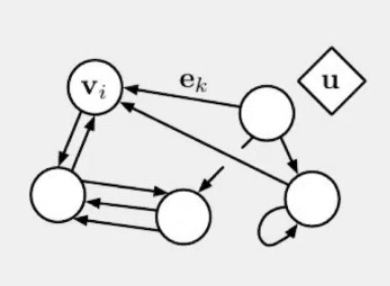
\includegraphics[width=0.32\textwidth]{figuresML/lesson_ml_5_pag_35.png}
\end{center}
\begin{itemize}
    \item[-] \textbf{Vertices/Nodes ($V$):} the fundamental entities of the graph. In a physical system, these could be planets, stars, or particles. Each node $v_i$ possesses \textbf{attributes} or \textit{features}, which hold the intrinsic information of the individual entities within the graph (e.g., mass, position, and velocity of the $i$-th body in the 3-body example).
    \item[-] \textbf{Edges ($E$):} the connections between vertices. Edges can be \textbf{directed} (one way) or \textbf{undirected} (bidirectional), and the number of edges connected to a specific vertex is called its \textbf{degree}. Edges $e_k$ represent relations or interactions, such as gravitational forces between bodies in our example or decay lineages between particles in other physical applications. \\
    Attributes can also be defined on the edges and once again, we can observe the enormous versatility of GNNs starting from our example: theoretically, given the positions of the bodies, we already possess all the information needed to deduce their mutual distances. We can therefore provide these as initial attributes on the edges, saving the GNN from spending resources and parameters to learn how to calculate them autonomously. Thus, we can decide to let the network learn to predict only the more complex relationships (e.g., the interaction forces between the bodies) to update the states of both nodes and edges, significantly improving its efficiency.
    \item[-] \textbf{Global state ($u$):} attributes that belong to the graph as a whole, rather than to any specific node or edge. Examples include the total energy or the overall angular momentum of a multi-body system. As outlined in the following figure, we can store the general properties of the graph in these global attributes.
\end{itemize}

\begin{center}
    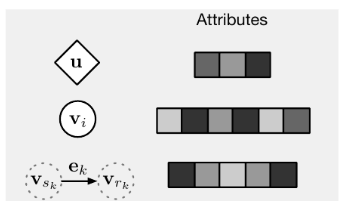
\includegraphics[width=0.4\linewidth]{figuresML/lesson_ml_5a_pag_8.png}
\end{center}

Just as CNNs apply the exact same convolutional kernel across different patches of an image, a GNN applies the exact same updating function to all nodes, one at a time. Because the function weights are shared, swapping node 1 with node 2 does not change the network's overall understanding of the system, perfectly preserving permutation equivariance. You will find much more detail at the following link: \url{https://arxiv.org/abs/1806.01261}.

\begin{figure}[H]
    \begin{minipage}[c]{0.75\textwidth}
        Graphs can be useful when your data is a list of values that would result in a sparse format if you try to bin it and put it on a grid (think for example about a jet of particles from LHC). Even if no actual link exists in sparse datasets, you can still use any type of clustering algorithm. For example, as long as some “distance” can be defined, a graph structure can be created looking at the $k$ nearest neighbors, where $k$ is a chosen integer, as represented in figure. Alternatively, if computational resources permit, we can initialize a fully connected graph where every node is linked to every other node.
    \end{minipage}\hfill
    \begin{minipage}[c]{0.25\textwidth}
        \centering
        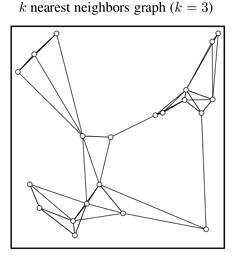
\includegraphics[width=0.9\linewidth]{figuresML/lesson_ml_5_pag_32.png}
    \end{minipage}
\end{figure}
\vspace{-7.5mm}

\subsection{Tasks on a Graph}
Depending on the specific goal of the analysis, GNNs are extremely versatile and can be applied to extract predictions at different levels of the graph hierarchy, as represented below:
\begin{itemize}
    \item[-] \textbf{Node-level tasks:} Predicting a label, type, or attribute for an individual node. An example in industry is detecting fake accounts within a massive social network; in physics, identifying the specific particle type of a given detector hit.
    \item[-] \textbf{Edge-level tasks:} Given a set of nodes, inferring missing edges or predicting the strength of a connection. For instance, predicting the probability that a user will buy a product, or in HEP, evaluating whether two separate particle tracks originated from the same primary vertex.
    \item[-] \textbf{Graph-level tasks:} Carrying out classification or regression over the entire graph. A classic example is predicting a molecule's overall toxicity based on its structural graph, or determining the total energy of a physical system.
\end{itemize}
\begin{center}
    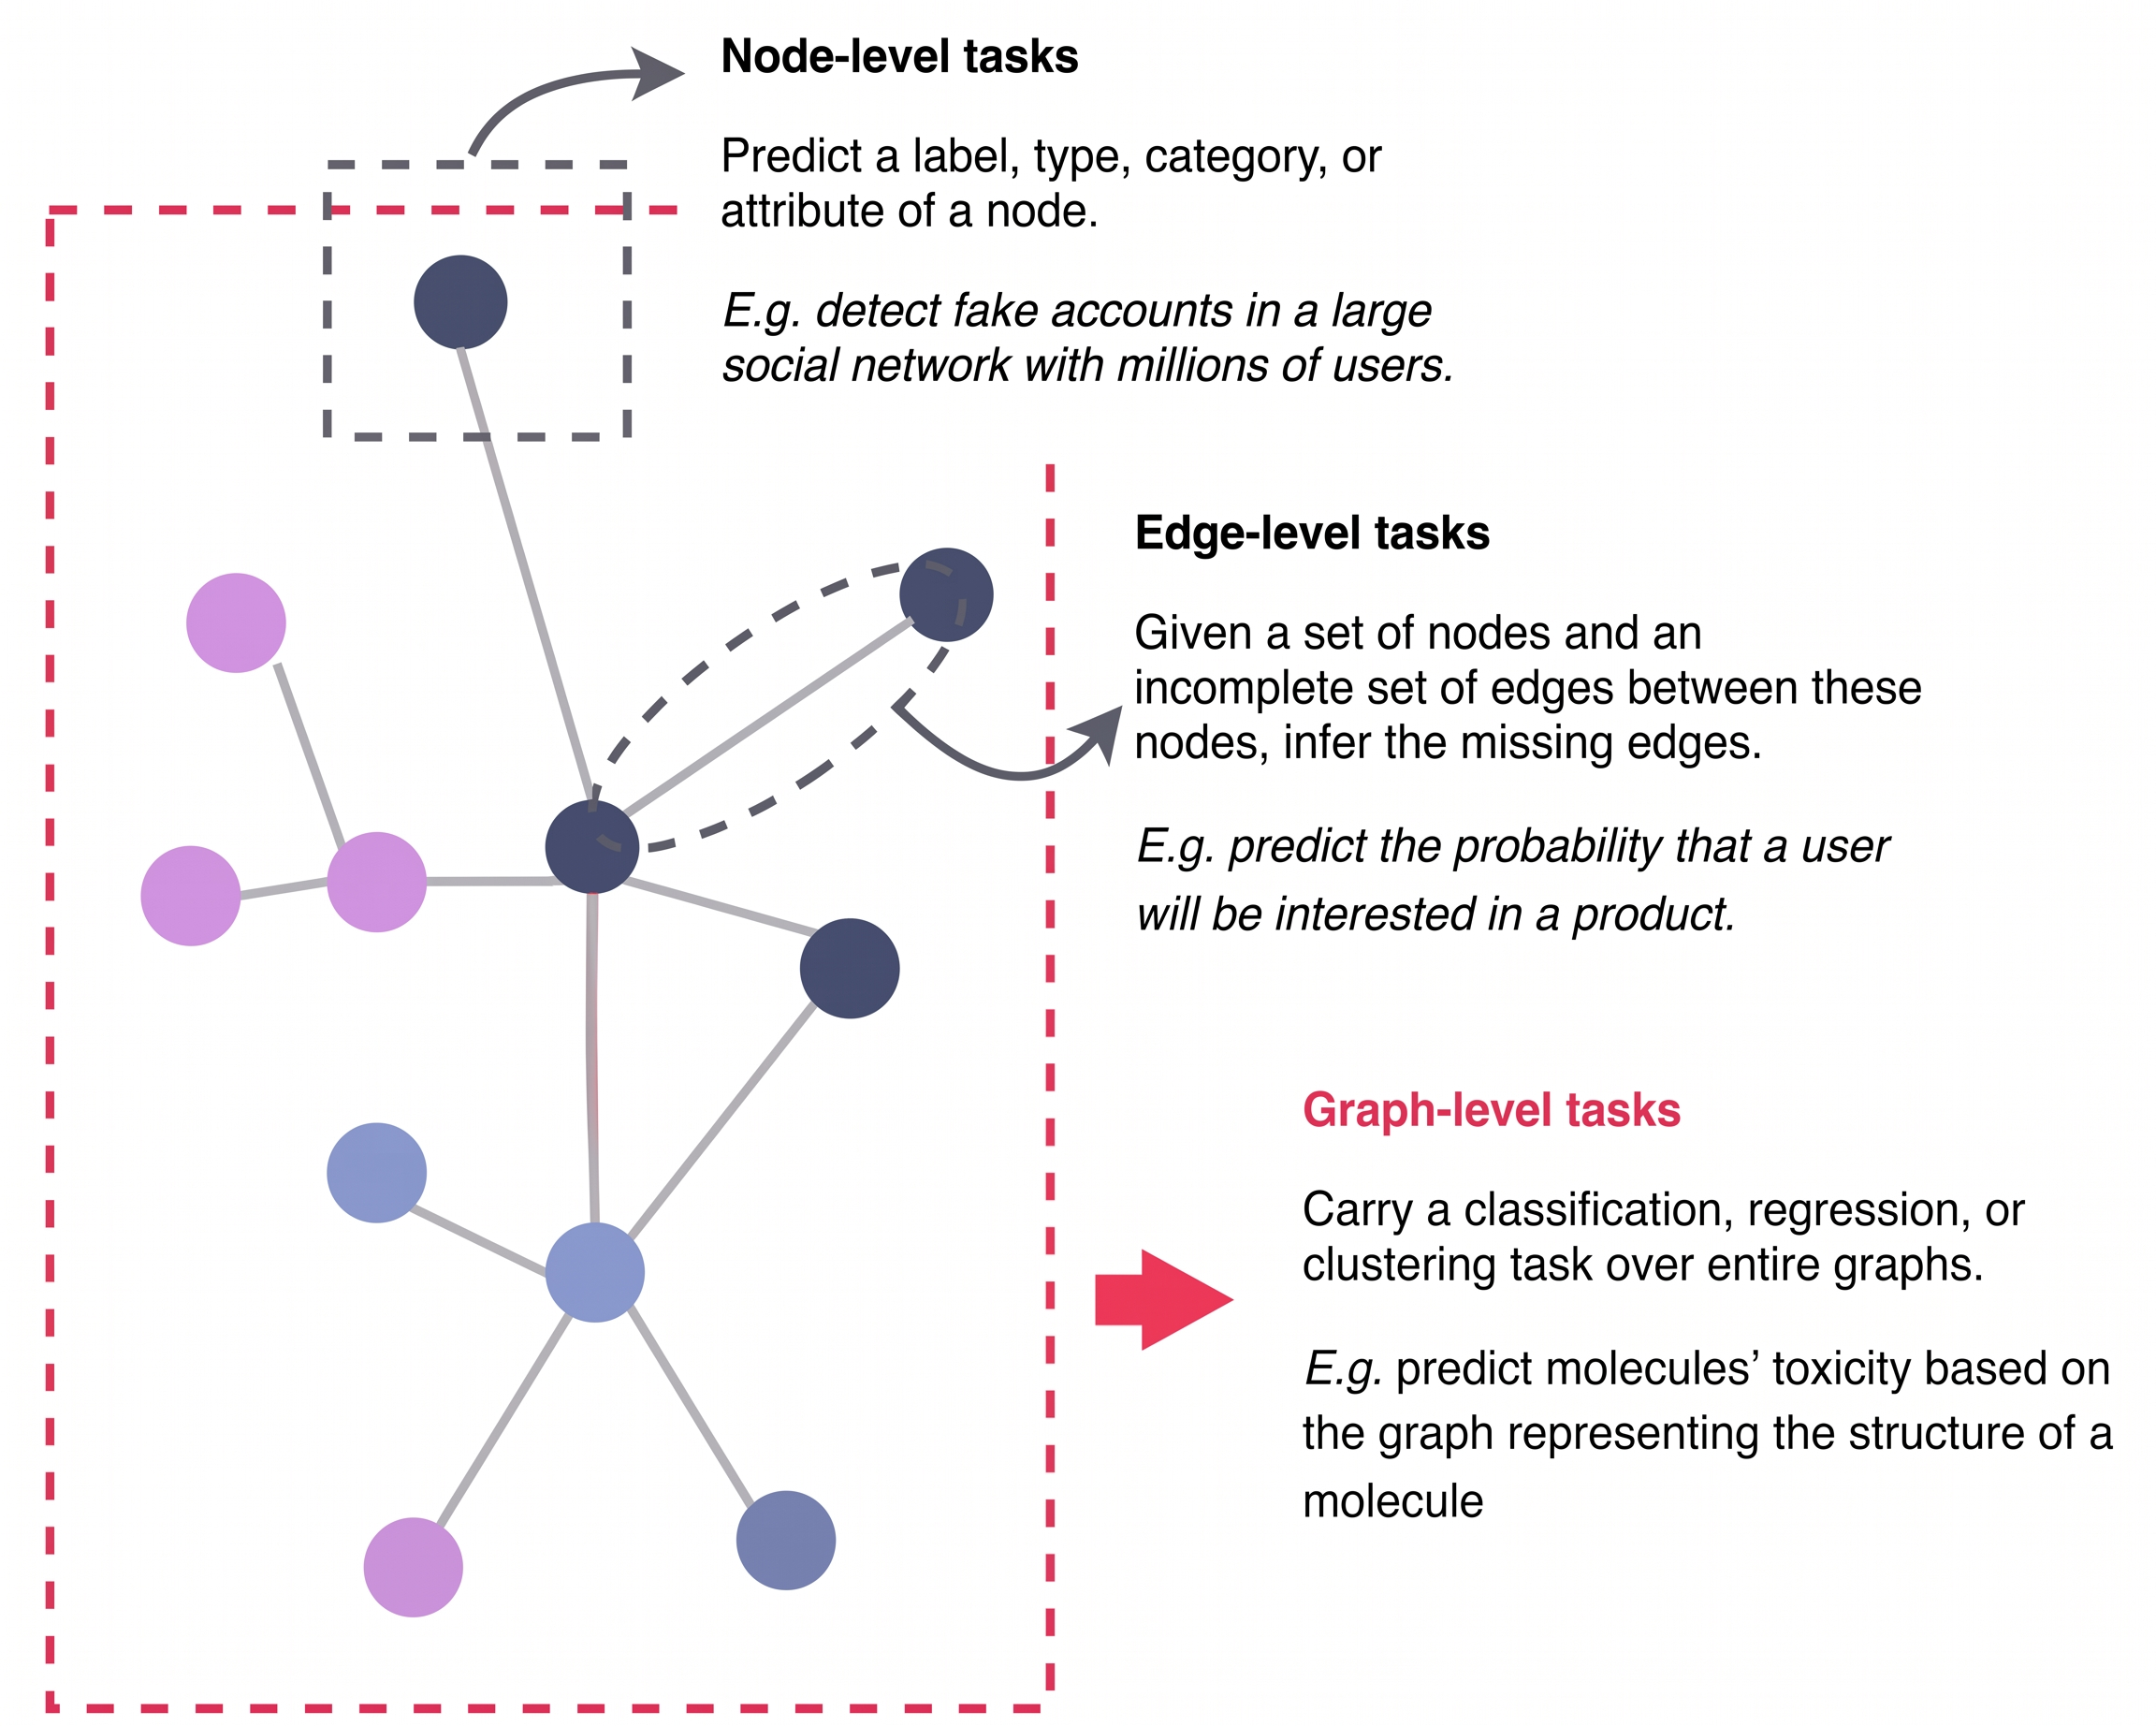
\includegraphics[width=0.45\linewidth]{figuresML/lesson_ml_5_pag_36.png}
\end{center}

\subsection{Building a GNN: Message Passing}
To solve these tasks, the GNN must learn new, richer representations for the nodes, edges, and global state. Just as a CNN extracts hierarchical features through successive convolutional layers, a GNN creates new features by mapping inputs to a high-dimensional latent space and iterating updates across the graph in a process called \textbf{Message Passing}. The mathematical logic follows a sequence of specific operations:

\textbf{1. The Embedding Phase:}
The raw input data typically resides in a physical space $X$, where features might represent concrete quantities like spatial coordinates or velocities. Let ${x_i}$ be the input vector of the node $v_i$ (e.g position, velocity, mass of a celestial body if your graph is representing an astrophysical system). Embedding consists in mapping ${x_i}$ (the physical data) into a higher dimensional vector 
\begin{equation}
    {h_i}=\phi_{\text{EMB}}({x_i})
\end{equation} 
that lies in a latent non-physical space $H$. ${h_i}$ is the so called \textbf{hidden} or \textbf{latent representation} of the node. Crucially, since the same embedding function (which is effectively an embedding neural network) is run over all the nodes, then permutation equivariance is preserved, just like a shared kernel assures translation equivariance for CNNs. 

\textbf{2. The Message Passing Mechanism:}
Once embedded in the high-dimensional latent space, the network updates each node's representation by letting it exchange information with its neighbors. This is the core of message passing, which can be broken down into generating messages, aggregating them, and updating the nodes:

\begin{itemize}
    \item \textbf{Edge Update (Message Generation):} First, information must be passed along the connections. In the absolute simplest scenario, the message on an edge connecting a sender to a receiver could just be a direct copy of the sender's latent vector. More generally, an edge neural network $\phi^e$ computes a message ${e}'_k$ based on the current edge features, the latent vectors of connected nodes, and potentially the global state ${u}$ of the network:
    \begin{equation}
        {e}'_k = \phi^e({e}_k, {h}_{r_k}, {h}_{s_k}, {u})
    \end{equation}
    \item \textbf{Aggregation:} A single node may receive multiple messages from various neighbors, since they might be connected to more than one edges. To process them, the network uses an \textbf{aggregator}, which is a permutation-invariant \textbf{pooling function} $\rho^{e \to v}$ (such as an element-wise sum, a max or a mean). This step effectively compresses the set of incoming message vectors ($E'_i$) into a single unified vector $\bar{{e}}'_i$ of the same dimensionality:
    \begin{equation}
        \bar{{e}}'_i = \rho^{e \to v}(E'_i)
    \end{equation}
    \item \textbf{Node Update:} The node must now synthesize its own current state with the summarized information from its neighbors. A node neural network $\phi^v$ takes the aggregated message $\bar{{e}}'_i$ and the node's current state ${h}_i$ to output the newly updated latent state ${h}'_i$:
    \begin{equation}\label{eq:node_update}
        {h}'_i = \phi^v(\bar{{e}}'_i, {h}_i, {u})
    \end{equation}
\end{itemize}
With that said, why do we need the higher dimensional latent space? \textit{Couldn't we have done it directly with the ${x_i}$ vectors?} The answer lies in the network's capacity to learn complex correlations and structural patterns. Raw physical features often reside in a low-dimensional space and possess heterogeneous units, making direct aggregation mathematically and physically inconsistent. By embedding $X$ into a higher-dimensional latent space, we provide the neural network with the necessary degrees of freedom to unravel non-linear relationships between a node and its neighborhood. Furthermore, in this abstract space, the message passing mechanism can safely aggregate information, combining learned representations rather than incompatible physical quantities and allowing the GNN to effectively cluster nodes based on task-specific similarities. In other words, by iterating this message passing procedure multiple times, nodes gather information from increasingly distant regions of the graph and, after training, nodes with similar relational roles or features will naturally cluster in similar regions of the latent space.

\textbf{3. Global Update (Optional):}
Finally, if the task requires an understanding of the entire system (a graph-level task), a global state can be updated. All updated edges ($E'$) and nodes ($V'$) are pooled into summary vectors:
\begin{align}
    \bar{{e}}' &= \rho^{e \to u}(E') \\
    \bar{{v}}' &= \rho^{v \to u}(V')
\end{align}
A global neural network $\phi^u$ then generates the updated global state ${u}'$:
\begin{equation}
    {u}' = \phi^u(\bar{{e}}', \bar{{v}}', {u})
\end{equation}

\subsection{Information propagation}
By applying the message passing operation multiple times, information flows across the graph. If we define $m$ as the number of message passing iterations, at $m=0$, a node only possesses its initial features. After $m=1$, a node incorporates information from its immediate neighbors. After $m=2$, the node updated representation inherently includes data from nodes two hops away, effectively increasing the receptive field of the network, as represented below. 
\begin{center}
    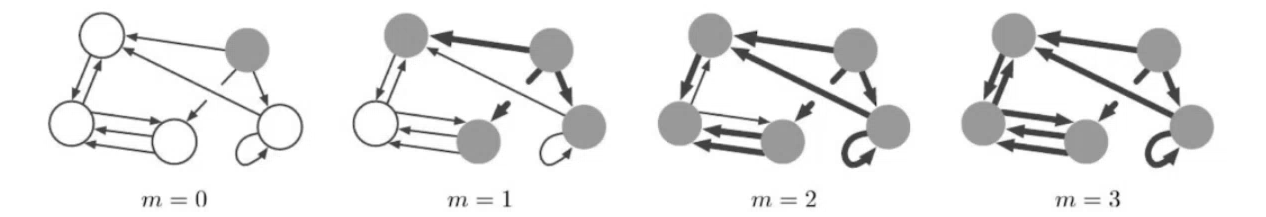
\includegraphics[width=0.8\linewidth]{figuresML/lesson_ml_5_pag_42.png}
\end{center}

\hrulefill

\textbf{Note:} Even though we will not treat them directly, it is worth mentioning the existence of so-called \textbf{heterogeneous graphs}. As shown in the previous diagram, two vertices can have more than one connection in the same direction. This implies that the edge will have two different hidden representations to transmit to the vertices. In practice, this means that the GNN operates as if there were two parallel graphs communicating in different ways. For instance, imagining that the vertices represent private users and companies, and that the algorithm is being used for market research, we might need to update the vertices belonging to the two categories differently. We will not go any further into this topic given its still limited applications in physics.

\hrulefill

Take a look at the following figure. The general algorithm described previously represents the most general possible form of a GNN, but message passing can be implemented in a variety of different ways depending on our specific needs. If, in our 3-body example, we only needed to compute the trajectory of body 3, it would make no sense to implement the updating of the global attributes. In the figure, we can observe different types of GNNs and message passing paradigms. Notice how a Deep-Set is essentially just a GNN without the edges.

\begin{center}
    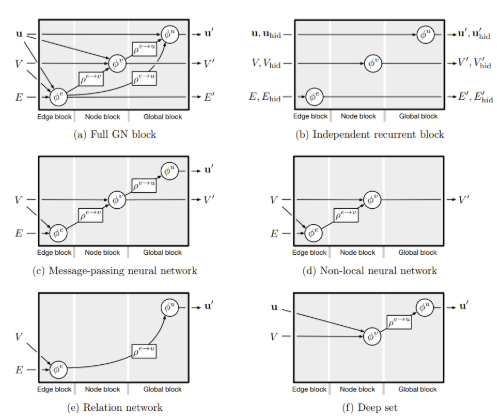
\includegraphics[width=0.7\linewidth]{figuresML/lesson_ml_5a_pag_15}
\end{center}


If the number of message passing steps is too large, or if the graph is fully connected without caution, the \textit{distinct signals from distant nodes can become severely diluted}. Therefore, choosing the correct graph connectivity (which is really an hyperparameter of the network, e.g., using $k$-NN) is essential to ensure the network receives direct and meaningful information. \\
You can find much more on the topic of GNNs in the following review article: \url{https://arxiv.org/abs/1806.01261}.

\subsection{Designing the Loss Function}
As we discussed in the previous sections, GNNs are incredibly versatile because they can handle tasks at the node, edge, and graph levels. But how do we actually train such a multi-faceted network? The answer is that you have total freedom to design a loss function tailored specifically to your physical problem.

Let's consider a practical example from High Energy Physics. When a quark is produced in a collider, it cannot exist in isolation due to the strong nuclear force; instead, it generates a "spray" of multiple particles. We can enclose this entire system in a "box" and represent it as a graph, where the input features are the kinematic properties (e.g., 4-momentum vectors) of the individual particles. If our main goal is a graph-level task (such as determining whether the original parent particle flew a certain distance before decaying or not) we are looking at a global classification problem. The GNN will embed the initial features, perform message passing to update the hidden representations, and finally apply a pooling function to extract a global vector $u'$. Passing $u'$ through MLP yields an output probability. We can then compute a standard \textit{graph-level loss} $\mathcal{L}_{graph}$ as a binary cross entropy.

However, what if we also want to extract local information? Suppose our simulation tells us that one specific particle in the jet is "special" (e.g., it carries a specific physical signature), and we want our network to accurately identify it. We can compute a \textit{node-level loss}, $\mathcal{L}_{node}$, by evaluating the output of the individual node representations.\\
Similarly, returning to our planetary example, if we wanted the network to predict the exact Newtonian force between pairs of planets, we would need to evaluate an \textit{edge-level loss}, $\mathcal{L}_{edge}$, working directly on the edge representations.

The true power of GNNs lies in the fact that these objectives are not mutually exclusive. If your problem requires it, \textit{you can train the network to solve all these tasks simultaneously by simply summing the individual loss components}:
\begin{equation}
    \mathcal{L}_{tot} = \mathcal{L}_{graph} + \mathcal{L}_{node} + \mathcal{L}_{edge}
\end{equation}
By doing so, the gradients backpropagating through the network will optimize the shared embedding and message passing layers to capture both the macroscopic properties of the system and the microscopic details of its individual constituents.

\subsection{Examples of application of GNNs}

\textbf{LHC Jet Tagging} \\
At the LHC, algorithms must quickly determine the origin of particle jets (e.g., identifying if a jet originated from a bottom quark, charm quark, or light quark). Because jets are point clouds, GNN architectures like CMS's \textit{ParticleNet} and ATLAS's \textit{GN1/GN2} have superseded older sequence-based models (like RNNs) and CNNs. These graph networks achieve dramatic improvements, such as a $\sim 5\times$ better background rejection rate when isolating specific decay channels.

\textbf{Global Weather Forecasting}\\
GNNs excel beyond particle physics. Google DeepMind \textit{GraphCast} models the Earth's atmosphere as a simultaneous multi-mesh graph to perform global weather forecasting. By passing messages across this massive spherical grid, it achieves predictions with similar or better accuracy than state of the art high-resolution numerical simulations (HRES) while operating significantly faster.

\subsection{Advanced Concepts: Attention Mechanisms and Dynamic Topologies}\label{sec:intro_att_mech}
While standard Message Passing Neural Networks are incredibly powerful, they traditionally treat the graph's connectivity as an \textit{a priori} hyperparameter. Furthermore, they update node representations without altering the underlying graph structure, which means that the number of nodes and edges remains strictly constant throughout the process. However, modern research and advanced physics applications often require much more flexible architectures.

Instead of hard-coding which nodes are connected using a binary incidence matrix (where elements are purely $1$ for an existing edge and $0$ for no edge), we can initialize a fully connected graph where everything is connected to everything. The goal then becomes to let the network itself learn the \textit{intent} or importance of each passing message. By promoting the binary matrix entries to continuous real numbers, the network dynamically assigns a higher weight to crucial messages and a lower weight to irrelevant ones. This self-learning of message importance is known as the \textbf{Attention Mechanism}. Instead of relying on a human-defined connectivity hyperparameter, the network becomes "attentive" to the specific connections that matter most for the given task. For example, this exact principle is at the very heart of Large Language Models (LLMs), where the network learns the relational importance between different words in a matrix representation of a sentence. We will see this in more detail in Sec. \ref{sec:transformers}.

Moreover, a standard GNN falls short when the task requires mapping an input graph of cardinality $M$ to an output of cardinality $N$, especially when $M \gg N$. A classic example in High Energy Physics is particle tracking: a small number of generated particles (cardinality $N$) might leave dozens of scattered hits (cardinality $M$) across different detector layers. A standard message passing block cannot intuitively reduce these $M$ reconstructed hits back to the $N$ original particles because it preserves the graph's initial dimensions.

To bypass this limitation, researchers are exploring generalized structures like \textbf{hypergraphs}, where hyperedges can connect multiple nodes simultaneously. Another highly effective, state of the art technique is \textbf{Object Condensation}. In this approach, the GNN maps the input nodes into the latent representation space, where we mathematically define interactive potentials. For example, we can introduce a "spring-like" attractive potential that pulls together latent objects belonging to the same physical source, alongside a repulsive potential for background noise or distinct particles. By minimizing this defined potential, the calculation naturally becomes the neural network's loss function, allowing the model to cluster relevant objects together and dynamically reconstruct the original particle sources.

\begin{comment}
\subsection{Advanced Concepts: Set-to-Set Problems and Attention}
While standard GNNs are extremely powerful, they are restricted to updating features without altering the underlying graph structure (the number of nodes and edges remains fixed). In complex tasks like particle tracking, where a network must map thousands of raw detector hits (cardinality $M$) to a handful of actual particle trajectories (cardinality $N$), a simple node update fails because $M \gg N$. 

To solve this, researchers use generalized structures like \textbf{hypergraphs} or a technique called \textbf{object condensation}. In object condensation, the GNN maps nodes into a latent space and defines artificial potentials. For example, a "spring-like" attractive potential pulls together nodes (hits) generated by the same source particle, while a repulsive potential pushes background noise away. Minimizing this potential natively clusters the graph, organically performing instance segmentation.

Another advanced approach to bypass hard-coded connectivity is the \textbf{Attention Mechanism}. Instead of relying on a binary incidence matrix ($1$ for connected, $0$ for not connected), we start with a fully connected graph and promote the connections to continuous real numbers. The neural network dynamically learns to assign weights to these edges, effectively deciding which messages are most important for the task. This self-learning of message importance forms the backbone of modern Transformer models.


\subsection{Practical Exercise: EdgeConv in PyTorch Geometric}
To solidify these concepts, the assignment uses the \texttt{PyTorch Geometric} library to classify point clouds as either circles or rectangles. Unlike standard images, you are provided only with $N$ un-ordered $(x,y)$ coordinates. 

Since the points lack edges, you must build the graph topology dynamically by computing the $k$-Nearest Neighbors ($k=10$). Once the graph is established, you will implement an \textbf{EdgeConv} layer. In this specific architecture, the edge message is generated by passing both the node's position and the relative distance vector between the two connected nodes through a trainable MLP, successfully extracting geometric features from an unstructured point cloud.
\end{comment}